\documentclass{article}
\usepackage[utf8]{inputenc}
\usepackage[margin = 0.8in]{geometry}
\usepackage{graphicx}
\usepackage{amsmath, amssymb}
\usepackage{subcaption}
\usepackage{multirow}
\usepackage{mathtools}
\usepackage{float}
\usepackage{enumitem}

\DeclareMathOperator*{\wrote}{Wrote}
\DeclareMathOperator*{\copyof}{CopyOf}
\DeclareMathOperator*{\owns2}{Owns}
\DeclareMathOperator*{\sings}{Sings}


\title{CS534 - HW 3}
\author{Keith Chester}
\date{Due date: July 10th 2022}

\begin{document}
\maketitle

\section*{Problem 1}

In this problem we are exploring $K$-means clustering.

We have a set of data representing five customer ratings on a new car, with a scale from 0 to 20. The image below represents that data:

\begin{figure}[H]
    \centering
    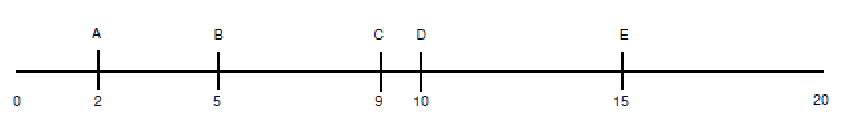
\includegraphics[width = 0.65\textwidth]{imgs/problem1_data.png}
\end{figure}

\subsection*{Part A}

Assuming that $K=2$, and the two initial centroids are $3$ and $4$, we will try to utilize the K-means algorithm to show all computational steps.

\begin{equation}
    K = [2, 5, 9, 10, 15];\; C_0 = 3;\;  C_1 = 4
\end{equation}

\noindent Next we find the distance (simple, since we're working with a singular dimension) from each point in order to assign it.

\begin{center}
    \begin{tabular}{c r r}
        Data point & Distance from $C_0$ & Distance from $C_1$\\
        2 & \textbf{1} & 2 \\
        5 & 2 & \textbf{1} \\
        9 & 6 & \textbf{5} \\
        10 & 7 & \textbf{6} \\
        15 & 12 & \textbf{11} \\
    \end{tabular}
\end{center}

\noindent Here we've bolded the closer distance to the associated centroid. We will now recompute the resulting centroid position by taking the mean value of all points assigned.

\begin{equation}
    C_i = \frac{1}{n} \sum_{x_i \rightarrow C_i} x_i
\end{equation}

\begin{equation}
    C_0 = \frac{1}{n} \sum_{x_i \rightarrow C_0} x_i = \frac{1}{1} \sum (2) = 2
\end{equation}

\begin{equation}
    C_1 = \frac{1}{n} \sum_{x_i \rightarrow C_1} x_i = \frac{1}{4} \sum (5,9,10,15) = 9.75
\end{equation}

\noindent This gives us two new centroids at $C_0=2$ and $C_1=9.75$. We continue this process until we no longer have any points change centroid assignments.

\begin{center}
    \begin{tabular}{c r r}
        Data point & Distance from $C_0$ & Distance from $C_1$\\
        2 & \textbf{0} & 7.75 \\
        5 & \textbf{3} & 4.75 \\
        9 & 7 & \textbf{0.75} \\
        10 & 8 & \textbf{0.25} \\
        15 & 13 & \textbf{5.25} \\
    \end{tabular}
\end{center}

\noindent ...since we have a new point on the first centroid, we run the calculations to get the new centroid averages again:

\begin{equation}
    C_0 = \frac{1}{n} \sum_{x_i \rightarrow C_0} x_i = \frac{1}{2} \sum (2,5) = 3.50
\end{equation}

\begin{equation}
    C_1 = \frac{1}{n} \sum_{x_i \rightarrow C_1} x_i = \frac{1}{3} \sum (9,10,15) = 11.33
\end{equation}

\noindent ...leaving us with $C_0=3.50$ and $C_1=11.33$. Continuing the process:

\begin{center}
    \begin{tabular}{c r r}
        Data point & Distance from $C_0$ & Distance from $C_1$\\
        2 & \textbf{0} & 9.33 \\
        5 & \textbf{3} & 6.333 \\
        9 & 5.50 & \textbf{2.33} \\
        10 & 6.50 & \textbf{0.67} \\
        15 & 11.50 & \textbf{3.67} \\
    \end{tabular}
\end{center}

\noindent Since we see no point changes, so our centroids are finalized at $C_0=3.50$ and $C_1=11.33$.

% SILHOUETTE INDEX

To find the Silhouette Coefficient Index, we take a given cluster $C_i$, select a point $x_i$ within it, and find the average distance distance between it and all other points within that cluster, which we'll mark as $a_1$. Then for each other cluster $C_j$, find the \textit{minimum} average distance ($a_j$) between this point and the average distance from each point in the other clusters.

\noindent ...choosing $x_i=x_0=2$ for our point

\begin{equation}
    a_1 = 3
\end{equation}

\noindent ...we need to test both $x_0$ and $x_1$ to find the minimum average distance to utilize for our calculation.

\begin{equation}
    a_2 = \frac{1}{n} \sum d(x_0, C_1); \; = \frac{1}{3} \sum (7, 8, 13) = 9.33
\end{equation}

\begin{equation}
    a_2 = \frac{1}{n} \sum d(x_1, C_1); \; = \frac{1}{3} \sum (4, 5, 10) = 6.33
\end{equation}


\noindent ...which, since we have only the one other cluster, we can stop here. We'll use the smaller $6.33$ average distance. If we had more clusters, we would take the minimum of the average distances from each point in other clusters, but we can stop here. We can now calculate the index $S_1$:

\begin{equation}
    S_1 = 1 - \frac{a_1}{a_2} = 1 - \frac{3}{6.33} = 0.53
\end{equation}

\noindent ...and then we do the same for the next cluster $C_2$. We use $x_i=x_3=9$.

\begin{equation}
    a_1 = \frac{1}{n} \sum d(x_2, C_1); \; = \frac{1}{2} (1, 6) = 3.5
\end{equation}

\noindent ...we need to test both $x_2$, $x_3$ and $x_4$ to find the minimum average distance to utilize for our calculation.

\begin{equation}
    a_2 = \frac{1}{n} \sum d(x_2, C_0); \; = \frac{1}{2} (7, 4) = 5.5
\end{equation}

\begin{equation}
    a_2 = \frac{1}{n} \sum d(x_3, C_0); \; = \frac{1}{2} (8, 5) = 6.5
\end{equation}

\begin{equation}
    a_2 = \frac{1}{n} \sum d(x_4, C_0); \; = \frac{1}{2} (12, 10) = 11
\end{equation}

\noindent ...using $a_2=5.5$ as our minimum.

\begin{equation}
    S_2 = 1- \frac{a_1}{a_2} = 1 - \frac{3.5}{5.5} = 0.37
\end{equation}

\noindent ...so the Silhouette Coefficient Index for our clusters $C_0$ and $C_1$ are $S_1=0.76$ and $S_2=0.37$, respectively.

% DAVIES BOULDIN INDEX

We are now going to calculate the Davies-Bouldin Index. To find this, we will be first finding the average distance from a given cluster's $C_i$'s points to its centroid ($s_i$), the distance between the centroids of two given clusters ($d_{ij}$), and then the max $R_{i,j}$ where...

\begin{equation}
    R_{i,j} = \frac{s_1+s_2}{d_{ij}}
\end{equation}

\noindent ...then we find the max $R_{i,j}$ (which will be the only one we calculate as we only have two clusters), and then take the average of those maxes - will again be just $R_{ij}$ given our setup.

\begin{equation}
    D_i = \max(R_{i,j})
\end{equation}

\begin{equation}
    DB_{index} = \frac{1}{N} \sum^N_{i=1} D_i
\end{equation}

\noindent ...and now with our values:

\begin{equation}
    s_1 = \frac{1}{2} \sum (1.5, 1.5) = 1.5
\end{equation}

\begin{equation}
    s_2 = \frac{1}{3} \sum (2.33, 1.33, 3.67) = 2.44
\end{equation}

\begin{equation}
    R_{0,1} = \frac{1.5 + 2.44}{7.83} = 0.50
\end{equation}

% CH INDEX

Finally we are moving onto the Calinski-Harabasz Index. To calculate this, we will be utilizing the following equation:

\begin{equation}
    CH = \left\lbrack \frac{\sum^K_{k=1} n_k \|c_k-C\|^2}{K-1} \right\rbrack / \left\lbrack \frac{\sum^K_{k=1} \sum^{n_k}_{i=1} \| d_i - c_k \|^2}{N-K}\right\rbrack
\end{equation}

\noindent ...where $CH$ is our index, $C$ is the global centroid, $K$ is the total number of clusters, $N$ is the number of points, and $d_i$ is a given data point within a cluster. $n_k$ and $c_k$ are the number of points within and the centroid of cluster $k$, respectively.

\begin{equation}
    C = \frac{1}{N} \sum (d_i) = \frac{1}{5} \sum (2,5,9,10,15) = 8.2
\end{equation}

\begin{equation}
    CH = \frac{\left\lbrack \frac{\sum (2\|3.5-8.2\|^2, 3\|11.33-8.2\|^2)}{1} \right\rbrack} { \left\lbrack \frac{\sum (\sum (\|2-3.5\|^2, \|5-3.5\|^2), \sum(\|9-11.33\|^2, \|10-11.33\|^2, \|15-11.33\|^2) )}{5-2} \right\rbrack}
\end{equation}

\begin{equation}
    CH = \frac{\left\lbrack \frac{\sum (2*22.09, 3*9.80)}{1} \right\rbrack} { \left\lbrack \frac{\sum (\sum (2.25, 2.25), \sum(5.43, 1.77, 13.47) )}{3} \right\rbrack}
\end{equation}

\begin{equation}
    CH = \frac{\left\lbrack \frac{\sum (44, 28.83)}{1} \right\rbrack} { \left\lbrack \frac{\sum (\sum (2.25, 2.25), \sum(5.43, 1.77, 13.47) )}{3} \right\rbrack}
\end{equation}

\begin{equation}
    CH = \frac{\left\lbrack \frac{72.83}{1} \right\rbrack} { \left\lbrack \frac{\sum(4.5, 20.67)}{3} \right\rbrack}
\end{equation}

\begin{equation}
    CH = \frac{\left\lbrack 72.83 \right\rbrack} { \left\lbrack \frac{25.17}{3} \right\rbrack}
\end{equation}

\begin{equation}
    CH = 8.68
\end{equation}

\subsection*{Part B}

We are doing that again, for some reason. This time, however, we'll be starting with the initial centroids of $11$ and $12$.


\begin{equation}
    K = [2, 5, 9, 10, 15];\; C_0 = 11;\;  C_1 = 12
\end{equation}

\noindent Next we find the distance (simple, since we're working with a singular dimension) from each point in order to assign it.

\begin{center}
    \begin{tabular}{c r r}
        Data point & Distance from $C_0$ & Distance from $C_1$\\
        2 & \textbf{9} & 10 \\
        5 & \textbf{6} & 7 \\
        9 & \textbf{2} & 3 \\
        10 & \textbf{1} & 2 \\
        15 & 4 & \textbf{3} \\
    \end{tabular}
\end{center}

\noindent Here we've bolded the closer distance to the associated centroid. We will now recompute the resulting centroid position by taking the mean value of all points assigned.

\begin{equation}
    C_i = \frac{1}{n} \sum_{x_i \rightarrow C_i} x_i
\end{equation}

\begin{equation}
    C_0 = \frac{1}{n} \sum_{x_i \rightarrow C_0} x_i = \frac{1}{4} \sum (2, 5, 9, 10) = 6.5
\end{equation}

\begin{equation}
    C_1 = \frac{1}{n} \sum_{x_i \rightarrow C_1} x_i = \frac{1}{1} \sum (15) = 15
\end{equation}

\noindent This gives us two new centroids at $C_0=6.5$ and $C_1=15$. We continue this process until we no longer have any points change centroid assignments.

\begin{center}
    \begin{tabular}{c r r}
        Data point & Distance from $C_0$ & Distance from $C_1$\\
        2 & \textbf{4.5} & 13 \\
        5 & \textbf{1.5} & 10 \\
        9 & \textbf{2.5} & 6 \\
        10 & \textbf{3.5} & 5 \\
        15 & 8.5 & \textbf{0} \\
    \end{tabular}
\end{center}

\noindent Since we see no point changes, so our centroids are finalized at $C_0=6.50$ and $C_1=15$.

% SILHOUETTE INDEX

Now let's calculate the Silhouette Coefficient Index. Choosing $x_i=x_0=2$ for our point

\begin{equation}
    a_1 = \frac{1}{3} \sum((5-2), (9-2), (10-2)) = 5.67
\end{equation}

\noindent ...we need to test $x_0$, $x_1$, $x2$, and $x_3$ to find the minimum average distance to utilize for our calculation.

\begin{equation}
    a_2 = \frac{1}{n} \sum d(x_0, C_1); \; = \frac{1}{1} (13) = 13
\end{equation}

\begin{equation}
    a_2 = \frac{1}{n} \sum d(x_1, C_1); \; = \frac{1}{1} (10) = 10
\end{equation}

\begin{equation}
    a_2 = \frac{1}{n} \sum d(x_2, C_1); \; = \frac{1}{1} (6) = 6
\end{equation}

\begin{equation}
    a_2 = \frac{1}{n} \sum d(x_3, C_1); \; = \frac{1}{1} (5) = 5
\end{equation}

\noindent ...which, since we have only the one other cluster, we can stop here. We'll use the minimum value of $5$ average distance. If we had more clusters, we would take the minimum of the average distances from each point in other clusters, but we can stop here. We can now calculate the index $S_1$:

\begin{equation}
    S_1 = 1 - \frac{a_1}{a_2} = 1 - \frac{5.67}{5} = -0.34
\end{equation}

\noindent ...and then we do the same for the next cluster $C_2$. We use $x_i=x_4=15$.

\begin{equation}
    a_1 = \frac{1}{1} \sum d(x_4, C_1); \; = \frac{1}{1} (0) = 0
\end{equation}

Since we have a 0, we can just stop here:

\begin{equation}
    S_2 = 1- \frac{a_1}{a_2} = 1 - \frac{0}{a_2} = 1 - 0 = 1
\end{equation}

\noindent ...so the Silhouette Coefficient Index for our clusters $C_0$ and $C_1$ are $S_1=-0.34$ and $S_2=1$, respectively.

% DAVIES BOULDIN INDEX

We are now going to calculate the Davies-Bouldin Index for this cluster outcome.

\begin{equation}
    R_{i,j} = \frac{s_1+s_2}{d_{ij}}
\end{equation}

\noindent ...then we find the max $R_{i,j}$ (which will be the only one we calculate as we only have two clusters), and then take the average of those maxes - will again be just $R_{ij}$ given our setup.

\begin{equation}
    D_i = \max(R_{i,j})
\end{equation}

\begin{equation}
    DB_{index} = \frac{1}{N} \sum^N_{i=1} D_i
\end{equation}

\noindent ...and now with our values:

\begin{equation}
    s_1 = \frac{1}{4} \sum (4.5, 1.5, 2.5, 3.5) = 3.0
\end{equation}

\begin{equation}
    s_2 = \frac{1}{3} \sum (0) = 0
\end{equation}

\begin{equation}
    R_{0,1} = \frac{3.0 + 0}{8.5} = 0.35
\end{equation}

% CH INDEX

Finally we move onto our last Calinski-Harabasz Index. Again, we aim to calculate:

\begin{equation}
    CH = \left\lbrack \frac{\sum^K_{k=1} n_k \|c_k-C\|^2}{K-1} \right\rbrack / \left\lbrack \frac{\sum^K_{k=1} \sum^{n_k}_{i=1} \| d_i - c_k \|^2}{N-K}\right\rbrack
\end{equation}

\begin{equation}
    C = \frac{1}{N} \sum (d_i) = \frac{1}{5} \sum (2,5,9,10,15) = 8.2
\end{equation}

\begin{equation}
    CH = \frac{\left\lbrack \frac{\sum (4\|6.5-8.2\|^2, 1\|15-8.2\|^2)}{1} \right\rbrack} { \left\lbrack \frac{\sum (\sum (\|2-6.5\|^2, \|5-6.5\|^2, \|9-6.5\|^2, \|10-6.5\|^2), \sum(\|15-15\|^2) )}{5-2} \right\rbrack}
\end{equation}

\begin{equation}
    CH = \frac{\left\lbrack \frac{\sum (4\|-1.7\|^2, 1\|6.2\|^2)}{1} \right\rbrack} { \left\lbrack \frac{\sum (\sum (\|-4.5\|^2, \|-1.5\|^2, \|2.5\|^2, \|3.5\|^2), \sum(\|0\|^2) )}{3} \right\rbrack}
\end{equation}

\begin{equation}
    CH = \frac{\left\lbrack \frac{\sum (4*2.89, 1*38.44)}{1} \right\rbrack} { \left\lbrack \frac{\sum (\sum (20.25, 2.25, 6.25, 12.25), \sum(0) )}{3} \right\rbrack}
\end{equation}

\begin{equation}
    CH = \frac{\left\lbrack \frac{\sum (11.56, 38.44)}{1} \right\rbrack} { \left\lbrack \frac{\sum (\sum (41.0), \sum(0) )}{3} \right\rbrack}
\end{equation}

\begin{equation}
    CH = \frac{\left\lbrack \frac{50}{1} \right\rbrack} { \left\lbrack \frac{41}{3} \right\rbrack}
\end{equation}

\begin{equation}
    CH = 3.67
\end{equation}

\subsection*{Part C}

In this quesiton, we are asked which initial clusters yielded better results. To determine this, we compare the indexes we calculated for each setup, which we'll label $A$ and $B$.

\begin{center}
    \begin{tabular}{l c c r}
        Index & $A$ & $B$ \\
        SI & 0.76,\; 0.37 & -0.34,\; 1 \\
        DHI & 0.50 & 0.35 \\
        CHI & 8.68 & 3.67 \\
    \end{tabular}
\end{center}

For the Silhouette Index, the higher the SCI, the more clustering improves. The SI for $A$ is higher than one of the values of $B$ but not both, and the negative index value is a poor sign. The lower DHI is better, so $B$ wins out slightly here. $A$ wins with the CHI index, since higher is better.

Since $A$ wins two of three indexes, we would say that $A$ is the better clustering attempt.

\section*{Problem 2}

In this problem we are performing Association Analysis (AA) on the following supermarket customer transactions:

\begin{center}
    \begin{tabular}{c c c c}
        Transaction (C) & Milk (M) & Eggs (E) & Bread (B) \\
        Customer 1 & 0 & 1 & 1 \\
        Customer 2 & 1 & 0 & 1 \\
        Customer 3 & 1 & 1 & 0 \\ 
        Customer 4 & 0 & 1 & 1 \\ 
        Customer 5 & 1 & 1 & 1 \\ 
        Customer 6 & 0 & 1 & 1 \\ 
        Customer 7 & 1 & 1 & 1 \\ 
    \end{tabular}
\end{center}

\subsection*{Part A}

First we will generate all the possible itemsets:

\begin{center}
    \begin{tabular}{c c c c}
        Itemset & Size & Frequency & Support \\
        M & 1 & 0 & $\frac{4}{7}$\\\\
        E & 1 & 0 & $\frac{6}{7}$\\\\
        B & 1 & 0 & $\frac{6}{7}$\\\\
        ME & 2 & 1 & $\frac{3}{7}$\\\\
        MB & 2 & 1 & $\frac{3}{7}$\\\\
        EB & 2 & 3 & $\frac{5}{7}$\\\\
        MEB & 3 & 2 & $\frac{2}{7}$\\\\
    \end{tabular}
\end{center}

\subsection*{Part B}

Assuming that our support threshold is $30\%$, here we will generate all possible associations; note that we're only including itemsets of size 2 and higher.

\begin{center}
    \begin{tabular}{c c c}
        Antecedent & Consequent & Confidence \\
        M & E & $\frac{support(M \cup E)}{support(M)} = \frac{3/7}{4/7} = 0.75$ \\\\
        M & B & $\frac{support(M \cup B)}{support(M)} = \frac{3/7}{4/7} = 0.75$ \\\\
        E & B & $\frac{support(E \cup B)}{support(E)} = \frac{5/7}{6/7} = 0.83$ \\\\
    \end{tabular}
\end{center}

\subsection*{Part C}

If our confidence threshold is above 70\%, then $1)$ Milk, therefore Eggs, $2)$ Milk, therefore Bread, and $3)$ Eggs, therefore Bread.


\end{document}